\documentclass[Main.tex]{subfiles}
\begin{document}
\section{Case Deletion Diagnostics for Variance Ratios}
In this section, case deletion diagnostics are used on the variance components of the model. Specifically the ratio of between subject variances and the within subject variances respecitvely.


\[ \mbox{BSVR} = \frac{\sigma^2_2}{\sigma^2_2} , \mbox{   } \mbox{WSVR} = \frac{d^2_2}{d^2_2} \]

These variance ratios are re-computed for each case removed, and may be analysed seperately or jointly for outliers.

\subsubsection{Methods for Identifying Outliers}
The Grubbs' Test for Outliers is a commonly used technique for assessing outlier in a univariate data set, of which there are several variants. The first variant of Grubb's test is used to detect if the sample dataset contains one outlier, statistically different than
the other values. The test statistic is based by calculating score of this outlier $G$ (outlier minus mean and divided
by sd) and comparing it to appropriate critical values. Alternative method is calculating ratio of
variances of two datasets - full dataset and dataset without outlier. 
%The obtained value called U is bound with G by simple formula.
The second variant is used to check if lowest and highest value are two outliers on opposite tails of
sample. It is based on calculation of ratio of range to standard deviation of the sample.
The third variant calculates ratio of variance of full sample and sample without two extreme observations.
It is used to detect if dataset contains two outliers on the same tail.

As there may be several outliers present, the Grubbs test is not practical. However an indication that a point being beyond the fences according to Tukey's 
specification for boxplots, ( i.e. greater than $Q_3 +1.5 \mbox{IQR}$ or less than $Q_1 - 1.5 \mbox{IQR}$), will suffice.

\subsubsection{Mahalanbis Distance}
Bivariate Analyses may be applied jointly to the both sets of data sets, e.g Mahalanobis distances.

The WSVR values are plotted against the corresponding BSVR values. Confidence Ellipses can be superimposed over the plot with minimal effort. Two ellipses are generated by this technique, a 50 \% and 97.5\% confidence ellipse respectively. Outlying cases are idenified by the plot. Subject 68 is evident

The subjects were ranked by Mahalanobis distance, with the top 10 being presented in the following table. Both sets of ratio are addtionally expressed as a ratio of the full model variance ratios. 
\begin{center}
\begin{tabular}{|c|c|c|c|c|c|}
	\hline
	Subject (u) &  MD & WSVR$_{(u)}$ & WSVR (\%) & BSVR$_{(u)}$   & BSVR (\%)     \\ \hline \hline
     68 & 44.7284   & 1.3615  & 0.9132   & 1.0353  & 0.9849 \\ \hline
    30 & 16.7228   & 1.5045  & 1.0092   & 1.1024  & 1.0487 \\ \hline
    71 & 11.5887   & 1.5210  & 1.0202   & 1.0932  & 1.0400 \\ \hline
    80 & 11.0326   & 1.4796  & 0.9925   & 1.0114  & 0.9621 \\ \hline 
    38 & 10.3671   & 1.5011  & 1.0069   & 1.0917  & 1.0385 \\ \hline 
    67 & 10.1940   & 1.4308  & 0.9598   & 1.0514  & 1.0002 \\ \hline
    43  & 7.6932   & 1.4385  & 0.9649   & 1.0511  & 0.9999 \\ \hline
    72  & 4.7350   & 1.4900  & 0.9995   & 1.0262  & 0.9762 \\ \hline
    48  & 4.4321   & 1.4950  & 1.0028   & 1.0280  & 0.9779 \\ \hline
    29  & 4.3005   & 1.4910  & 1.0001   & 1.0769  & 1.0244 \\ \hline
\end{tabular} 
\end{center}
From this table one may conclude that subjects 72, 48 and 29 are not particularly influential. Interestingly Subject 78, which was noticeable in the case deletion diagnostics for fixed effects, does not feature in this table.

\begin{figure}[h!]
\centering
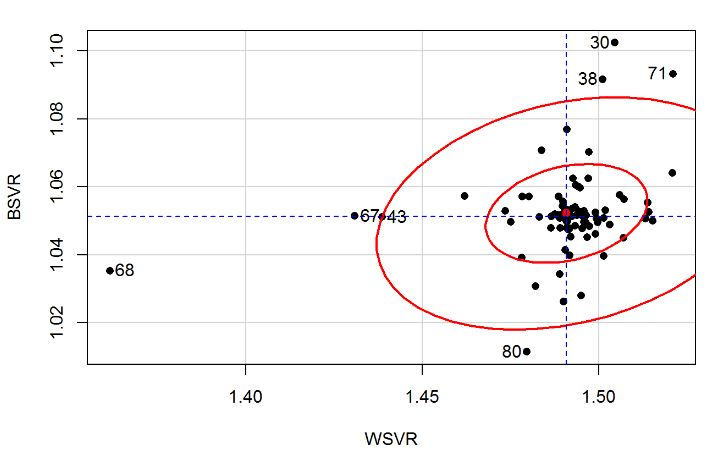
\includegraphics[width=0.9\linewidth]{08-plot1}
\caption{}
\label{fig:08-plot1}
\end{figure}

\end{document}

